%!TEX root = ../mtrgrmetod.tex
\chapter*{Вступ}

%На початку грудня 2020 року сервіс спільної розробки ІТ-проектів GitHub опублікував рейтинг найпопулярніших мов програмування, з якими працюють користувачі платформи. Перше місце зберіг \texttt{JavaScript}, слідом розташувався \texttt{Python}, третє місце займає \texttt{Java}, а на четверту сходинку піднявся \texttt{TypeScript}. П'яте місце залишається за \texttt{С\#},  далі йдуть \texttt{PHP}, \texttt{C++}, \texttt{C}, \texttt{Shell} і \texttt{Ruby}. З 2017 року склад першої десятки зберігається без змін, але \texttt{PHP} і \texttt{Ruby}, що знаходилися на вершині списку п'ять років тому, продовжують втрачати популярність.

%За результатами досліджень TIOBE \footnote{Рейтинг языков программирования TIOBE: январь 2020. [Електронний реурс]. -- 2020. -- Режим доступу: https://pr-cy.ru/news/p/7809-reyting-yazykov-programmirovaniya-tiobe-yanvar-2020} проведених у 2019 році мова \texttt{C} показала зростання популярності на 2,4 \%, і посіла перше місце, як первпективна для використання. Для порівняння \texttt{Python} в тому ж році показав зростання популярності лише на 1,4 \%. За тією ж оцінкою рейтинг мов програмування у 2020 році  виглядає наступним чином:

%1. \texttt{Java}; 2. \texttt{C}; 3. \texttt{Python}.

%\noindent
%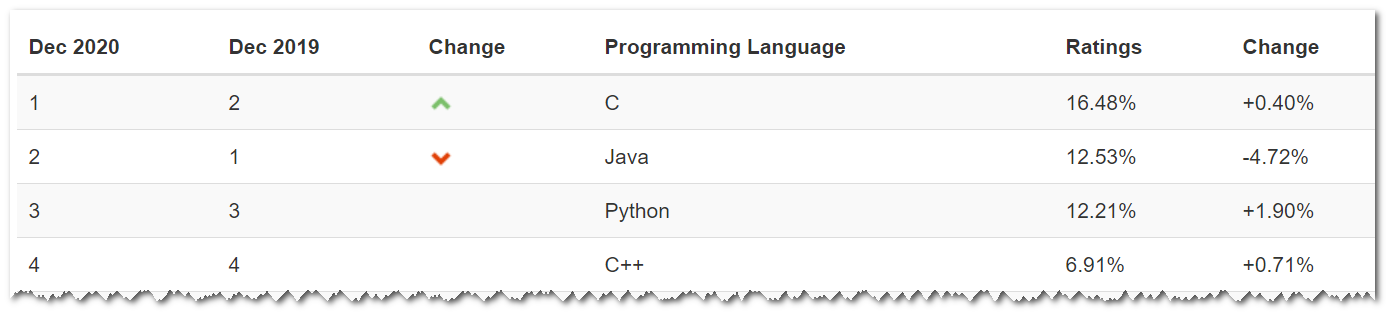
\includegraphics[width=\textwidth]{img/TIOBE_rating.png}

%Такою популярністю мова \texttt{C} зобов'язана концепції IoT (\textit{Internet of Things}) -- концепції мережі передачі даних між фізичними об'єктами («речами»), які обладнані вбудованими засобами та технологіями для взаємодії один з одним або із зовнішнім середовищем. Мова \texttt{C} підходить якнайкраще для створення невеликих пристроїв, яким вкрай важлива продуктивність за умови доступності вкрай обмежених апаратних ресурсів як об'єм пам'яті, обчислювальна потужність процесора тощо. 


%Актуальність вивчення дисципліни «Мікропроцесорна техніка» обумовлена необхідністю подальшого застосування в професійній діяльності фахівцями відповідних кваліфікацій знань і умінь в області апаратної реалізації і програмування мікропроцесорних засобів, програмних та апаратних інтерфейсів.
%
%Метою викладання навчальної дисципліни є формування знань в області мікропроцесорної техніки, що дозволяють аналізувати і проектувати мікропроцесорні пристрої.
%
%Публікація висвітлює один з аспектів проблеми проектування мікропроцесорних систем «без прив'я\-зу\-ван\-ня» до конкретного сімейства мікропроцесорів. Поданий матеріал орієнтований на вузьке коло студентів, які мають лише загальне уявлення про основи електроніки та схемотехніки, а при викладенні матеріалу використовується гіпотетичний мікропроцесор та пристрої зберігання інформації, які мають типові характристики  пристроїв, що випускаються в теперешній час.

%Розрахунково-графічна робота виконується студентами самостійно під керівниц\-твом викладача і для успішного її виконання важливим є вивчення нав\-чаль\-ної та методичної літератури з дисципліни «Мікропроцесорна техніка».

%Пропоновані методичні вказівки містять необхідну інформацію, яка сприятиме самостійному та грамотному виконанню розрахунково-графіч\-ної роботи. У відповідних розділах подано зміст і методику виконання розрахунків, завдання, порядок виконання та вимоги до оформлення текстової та графічної частини. Використовуючи рекомендований методичний підхід, студент зможе провести всі етапи проектування запам'ятовуючого пристрою для мікропроцесорної системи від постановки задачі до створення технічної документації.

«Мікропроцесорна техніка» є нормативною дисципліною в системі підготовки бакалавра, яка забезпечує теоретичну та практичну підготовку студентів для розв’язування фахових інженерних задач, а також використання спеціалізованого програмного забезпечення в процесі вив\-чен\-ня інших дисциплін, виконання курсових та дипломних робіт. Вивчення основ мікропроцесорної техніки ґрунтується на теоретичних положеннях курсу комп'ютерної техніки, програмування та алгоритмізації.

Дисципліна належить до тих фундаментальних дисциплін, які розвивають у студентів практичні навички, що стануть в пригоді як в процесі навчання, так і в професійній діяльності молодого фахівця. Основна задача курсу -- дати студентам знання у сфері застосування сучасних інформаційних технологій, забезпечити фундаментальність освіти майбутніх фахівців, а також навчити самостійно обирати та використовувати сучасний комп’ютерний інструментарій для вирішення фахових завдань. Знання та практичний досвід, набуті в процесі вивчення дисципліни, дозволять розширити можливості студентів при засвоєнні інших спеціальних дисциплін. 

\textit{Метою} навчальної дисципліни «Мікропроцесорна техніка» є розвиток алгоритмічного мислення, вивчення теоретичних основ і практичних засад проектування програмного забезпечення з використанням мов програмування низького рівня; отримання практичних навичок створення мікропроцесорних систем; набуття навичок роботи зі спеціалізованим програмним забезпеченням, трансляції програм в машинні коди, компонування машинного коду в пам'яті мікропроцесорної системи.

\textit{Предметом} вивчення дисципліни є проектування алгоритмів вирішення обчислювальних задач; створення програм та отримання машинного коду, придатного до вконання конкретним мікророцесором; ство\-рен\-ня елементарної мікропроцесорної системи, здатної виконувати елементарні обчислювальні завдання, оформлені відповідним чином.

Розрахунково-графічна робота з дисципліни «Мікропроцесорна техніка» є невід’ємною частиною навчального процесу, в ході виконання якої студенти набувають не лише необхідних навичок самостійної роботи, а й безпосередньо беруть участь у вирішенні практичних технічних задач. Метою даних методичних вказівок є викладення основних вимог до виконання та оформлення розрахунково-графічної роботи.